\section{O que é um Cluster}
Um Cluster é um grupo de computadores interligados que trabalham em conjunto para apoiar aplicações e middleware (por exemplo, \ac{BD}). Num Cluster, cada computador é referido como um "nó" ou \textit{node}. Ao contrário dos computadores de rede, em que cada nó executa uma tarefa diferente, os clusters de computadores atribuem a mesma tarefa a cada nó. Os nós de um cluster estão normalmente ligados entre si através de redes locais de alta velocidade. Cada nó executa a sua própria instância de um sistema operativo.

Os Clusters são frequentemente utilizados para \ac{HPC} e \ac{HA}. Se um único componente falhar num Cluster, os outros nós continuam a operar e a fornecer todo o processamento.
Os clusters são normalmente dedicados a funções específicas, tais como alta disponibilidade, alto desempenho ou processamento em grande escala.

\section{O que é um Galera Cluster}
Galera Cluster é um cluster de \ac{BD} multi-master baseado em replicação síncrona. Quando o Galera Cluster está em uso, as leituras e gravações da \ac{BD} podem ser dirigias a qualquer nó. Qualquer nó individual pode ser perdido sem interrupção nas operações e sem utilizar procedimentos complexos de \textit{failover}.

\subsection{Replicação Galera Cluster}
O Galera Cluster consiste num servidor de base de dados (MySQL ou MariaDB) que utiliza o plugin de Replicação Galera para gerir a replicação. O \ac{API} do plugin de replicação MySQL foi criada para fornecer toda a informação para uma replicação multi-master e síncrona. Esta \ac{API} é chamada de \ac{WSREP} API. 

\begin{figure}[H]
\center
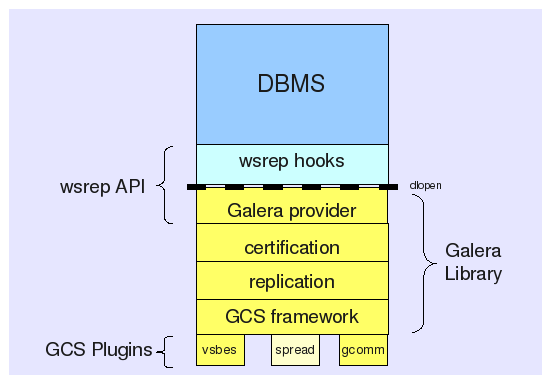
\includegraphics[width=12cm]{wsrep_api.png}
\caption{wsrep API}
\end{figure}

Através do \ac{WSREP} API, o Galera Cluster replica, entre todos os nós, a mesma informação mantendo todos os nós o mais atualizado possível. Mesmo que um nó deixe de ficar operacional os restantes assumem o papel para não comprometer o serviço e quando esse nó voltar a entrar no ativo recebe toda a informação que deixou de receber. A isto se chama uma replicação síncrona.

\subsection{Masters and Slaves}

Existem 2 modos de replicação no sistema de gestão de base de dados, \textit{Master-Slave} ou \textit{Multi-Master}. 
No modo \textit{Master-Slave} o servidor da base de dados principal regista as atualizações dos dados e propaga esses registos através da rede para os \textit{slaves}. Os servidores de base de dados de \textit{slaves} recebem um fluxo de atualizações do \textit{master} e aplicam essas alterações.

\begin{figure}[H]
\center
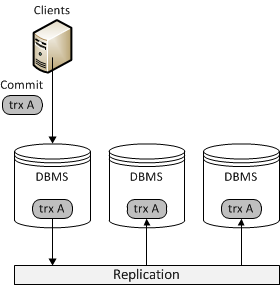
\includegraphics[width=8cm]{MS1.png}
\caption{Master-Slave}
\end{figure}

No modo \textit{Multi-Master}, todos os nós de \ac{BD} funcionam como \textit{master}. É possível submeter atualizações a qualquer nó da \ac{BD} porque estas se propagam através da rede para todos os nós.

\begin{figure}[H]
\center
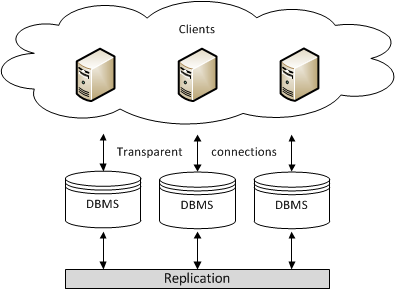
\includegraphics[width=10cm]{MS2.png}
\caption{Multi-Master}
\end{figure}

\subsection{Replicação Síncrona e Assíncrona}

Replicação síncrona não é nada mais do que todos os nós do cluster receberem a atualização que aconteceu num determinado nó. Ou seja, qualquer que seja a alteração feita num dos nós do cluster, todos os restantes vão receber imediatamente a atualização.

Replicação assíncrona não garante que a replicação chegue a todos os nós, tanto em tempo útil quanto a disponibilidade. A replicação assíncrona pode ser curta ou longa e implica também se um nó \textit{master} falhar, algumas das atualizações podem ser perdidas.